% !TEX encoding = UTF-8
% !TEX TS-program = pdflatex
% !TEX root = ../tesi.tex

%**************************************************************
\chapter{Progettazione}
\label{cap:progettazione-codifica}

In questo capitolo vengono presentati gli aspetti più interessanti della progettazione di \textit{moviORDER}. Il capitolo inizia con la descrizione dell'architettura generale della piattaforma, per poi entrare nel dettaglio delle varie componenti che la costituiscono.

\section{Architettura generale}

L'obiettivo di una buona progettazione è il soddisfacimento dei requisiti mediante un sistema di qualità, ottenibile tramite la definizione di una buona architettura logica del prodotto, che presenti componenti dalle specifiche chiare e coese, che sia realizzabile con risorse e costi fissati e che abbia una struttura che faciliti i cambiamenti futuri. In quest'ottica \textit{moviORDER} presenta un'architettura \textit{client-server}, dove il \textit{client} è l'applicazione installata sul dispositivo (\textit{Android} o \textit{iOS}) dell'utente finale, e il \textit{server} è un \textit{server web} \textit{Apache Tomcat} installato su un \textit{server Azure} di \visione{}. L'applicazione si connette al \textit{server} per la fruizione di un'\textit{API} che permette l'accesso a \textit{database} contenenti i dati di \textit{moviORDER}. Viene di seguito fornita una figura illustrativa dell'architettura generale della piattaforma.

\newpage

\begin{figure}[!h] 
    \centering 
    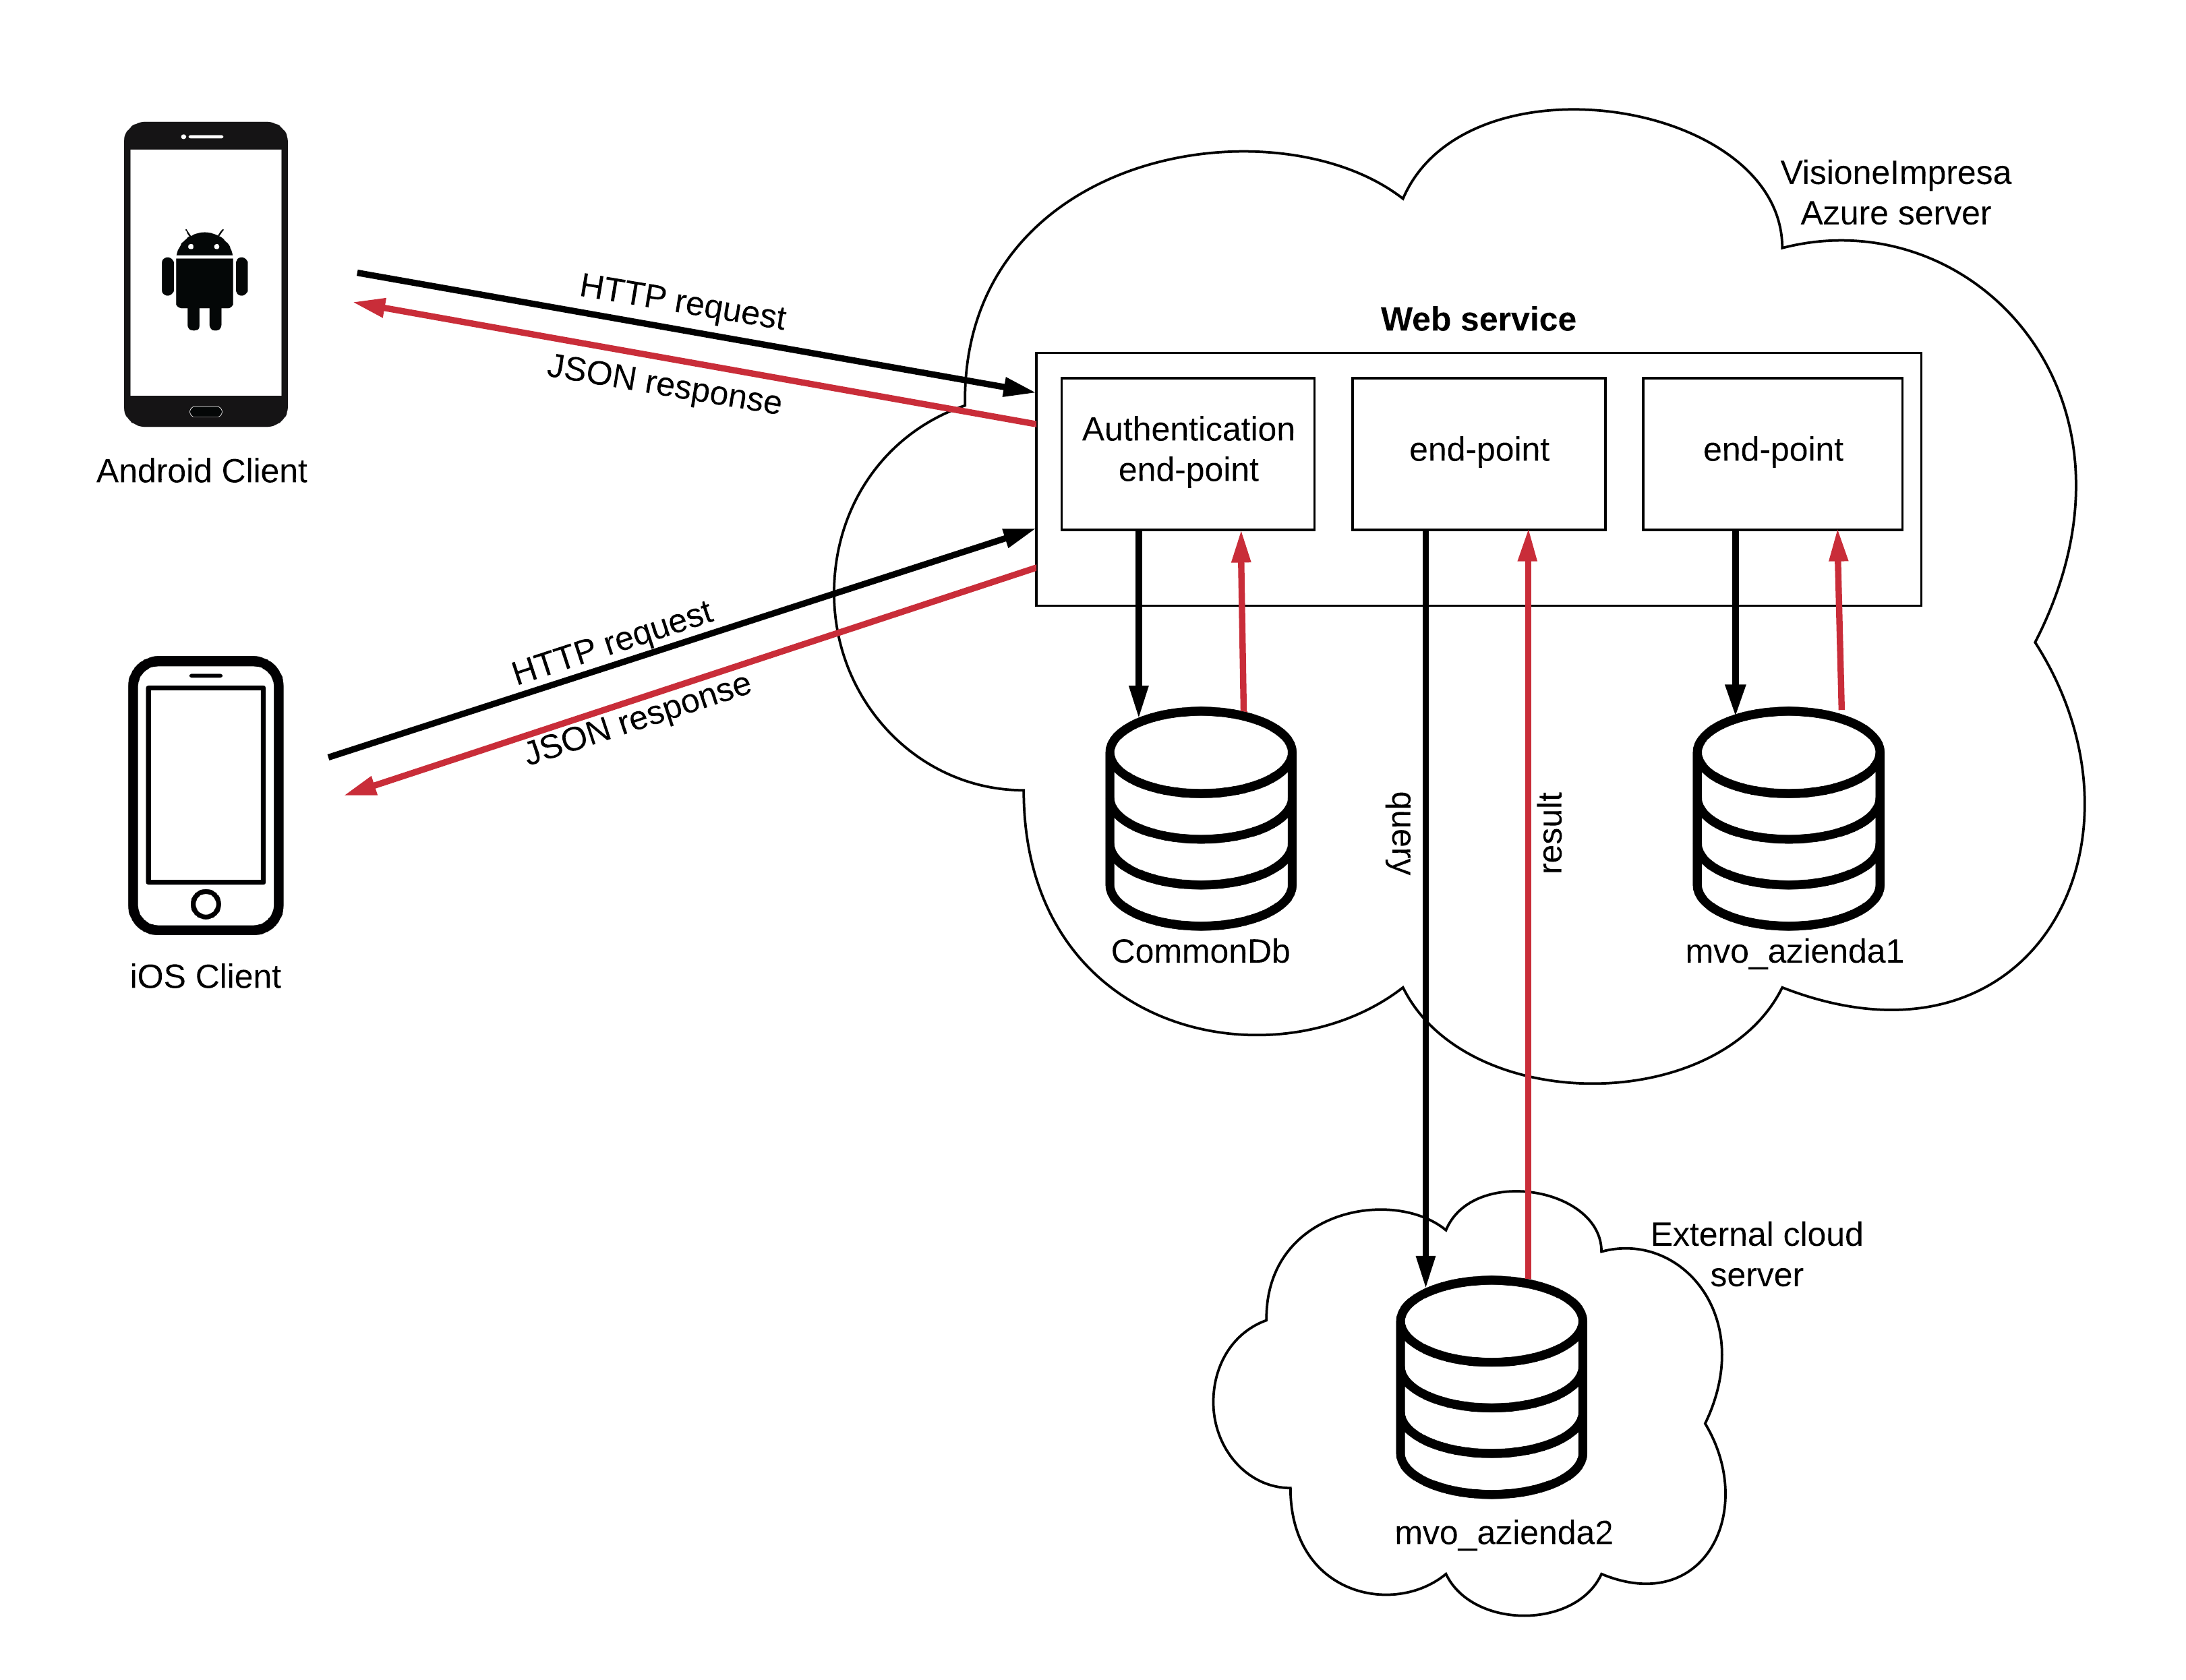
\includegraphics[width=\columnwidth]{progettazione/generalArchitecture} 
    \caption{Architettura generale di \textit{moviORDER}}
\end{figure}

L'applicazione comunica con il \textit{server} tramite l'invio di richieste \textit{HTTP}. Sul \textit{server} è installato un servizio \textit{web} che si occupa di elaborare tali richieste mediante oggetti \textit{servlet Java}, i quali eseguono delle \textit{query} sul \textit{database} e rispondono, sulla base dei risultati ottenuti, tramite stringhe codificate in formato \textit{JSON}. Per la costruzione delle risposte il servizio \textit{web} interroga i seguenti \textit{database} \textit{SQL Server}:
\begin{itemize}
	\item \textit{CommonDb}: \textit{database} locale al \textit{server Azure} di \visione{} e contenente i dati di autenticazione degli utenti di \textit{moviORDER}. Ogni qualvolta che un'azienda acquista il servizio, vengono inserite nel \textit{CommonDb} le credenziali di tutti gli utenti della stessa;
	\item \textit{mvo\_aziendaNomeAzienda}: \textit{database} contenente i dati utili alla gestione degli ordini presso l'azienda \textit{NomeAzienda}. All'interno del \textit{server Azure} è presente un \textit{database} di questa tipologia per ogni azienda che usufruisce del servizio e che ha deciso di affidare la gestione completa dei propri ordini a \visione{}. Per le aziende che preferiscono invece gestire internamente i propri ordini, tale \textit{database} è contenuto nei \textit{server cloud} delle stesse. Ne consegue che il servizio \textit{web} deve essere in grado di collegarsi a \textit{database} locali o remoti.
\end{itemize}
Una descrizione più approfondita dei dati contenuti in questi \textit{database} è presente in sezione §\ref{progdb}.

\subsection{Architettura \textit{front end}}

Sul \textit{client}, ovvero l'applicazione installata sul dispositivo dell'utente utilizzatore, è presente il \textit{pattern} architetturale \glossaryItem{MVP} (\textit{Model View Presenter}). Tale \textit{pattern} presenta componenti distribuite, infatti la \glossaryItem{view} e il \glossaryItem{presenter} si trovano sul dispositivo, mentre il \glossaryItem{model} si trova sul \textit{server Azure} di \visione{} o sul \textit{server cloud} di un'azienda cliente. Nello specifico, la \textit{view} è la \glossaryItem{GUI} (\textit{Graphical User Interface}) dell'applicazione, il \textit{presenter} è la logica applicativa della stessa, mentre il \textit{model} è il \textit{database} contenente i dati utili alla gestione degli ordini. È stato scelto un \textit{MVP} in quanto il \textit{model} interagisce solamente con il \textit{presenter}, e non può modificare la \textit{view} come invece accade per il \textit{pattern} \glossaryItem{MVC} (\textit{Model View Controller}). Nella seguente figura è possibile notare le differenze concettuali tra i due \textit{pattern}.

\begin{figure}[!h] 
    \centering 
    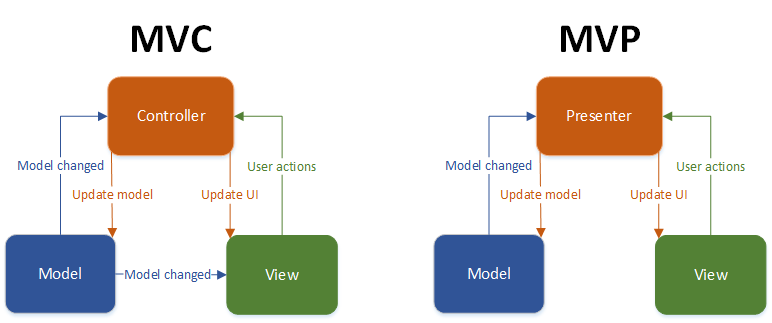
\includegraphics[width=\columnwidth]{progettazione/differenzepattern} 
    \caption{Differenze tra \textit{pattern} \textit{MVC} e \textit{MVP}}
\end{figure}

Viene di seguito presentata una figura illustrativa di come il design \textit{pattern} \textit{MVP} è stato istanziato nel \textit{front end} di \textit{moviORDER}.

\begin{figure}[!h] 
    \centering 
    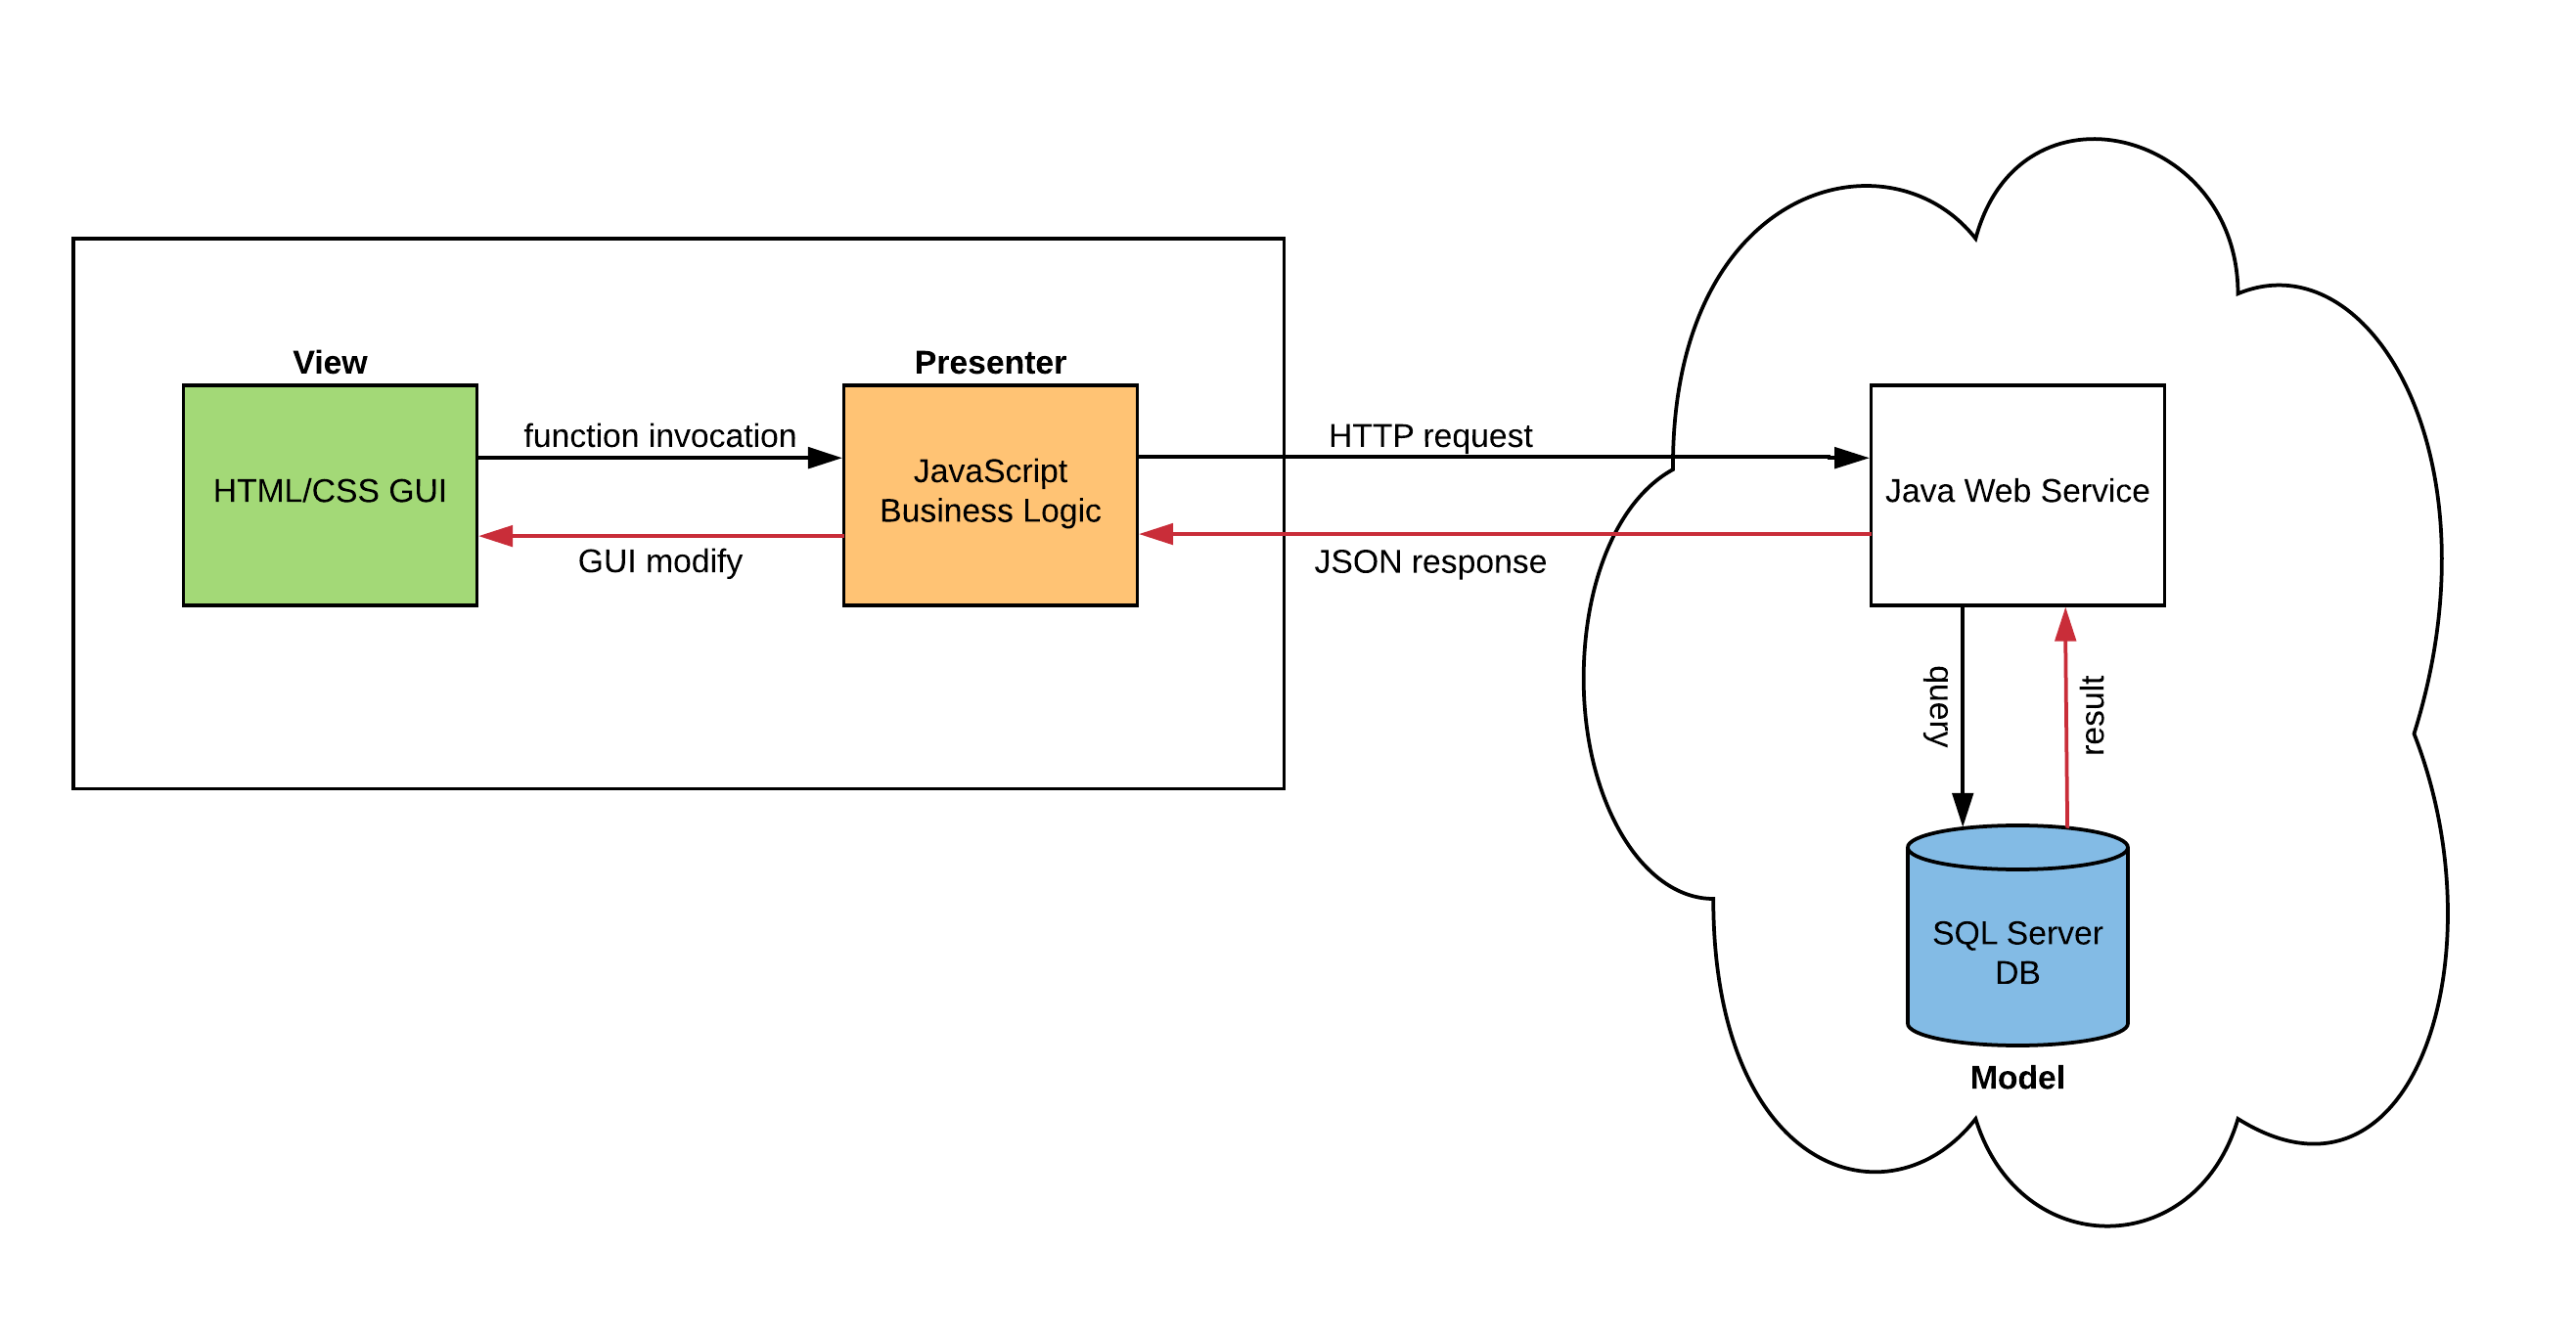
\includegraphics[width=\columnwidth]{progettazione/frontendMVP} 
    \caption{Architettura \textit{front end}}
\end{figure}

Nello specifico, il flusso del \textit{pattern} è il seguente:
\begin{itemize}
	\item l'utente interagisce con la \textit{view} eseguendo delle operazioni sull'interfaccia dell'applicazione;
	\item il \textit{presenter} capta le interazioni e, sulla base di queste, richiede la lettura/scrittura di dati sul \textit{model} tramite l'invio di richieste \textit{HTTP} ad un servizio \textit{web};
	\item il servizio \textit{web} legge/scrive sul \textit{model} a seconda della richiesta ricevuta, e prepara ed invia una risposta al presenter;
	\item il \textit{presenter} riceve la risposta, la elabora e modifica la \textit{view} di conseguenza.
\end{itemize}
Viene di seguito presentato un diagramma di sequenza che illustra il flusso appena descritto.

\begin{figure}[!h] 
    \centering 
    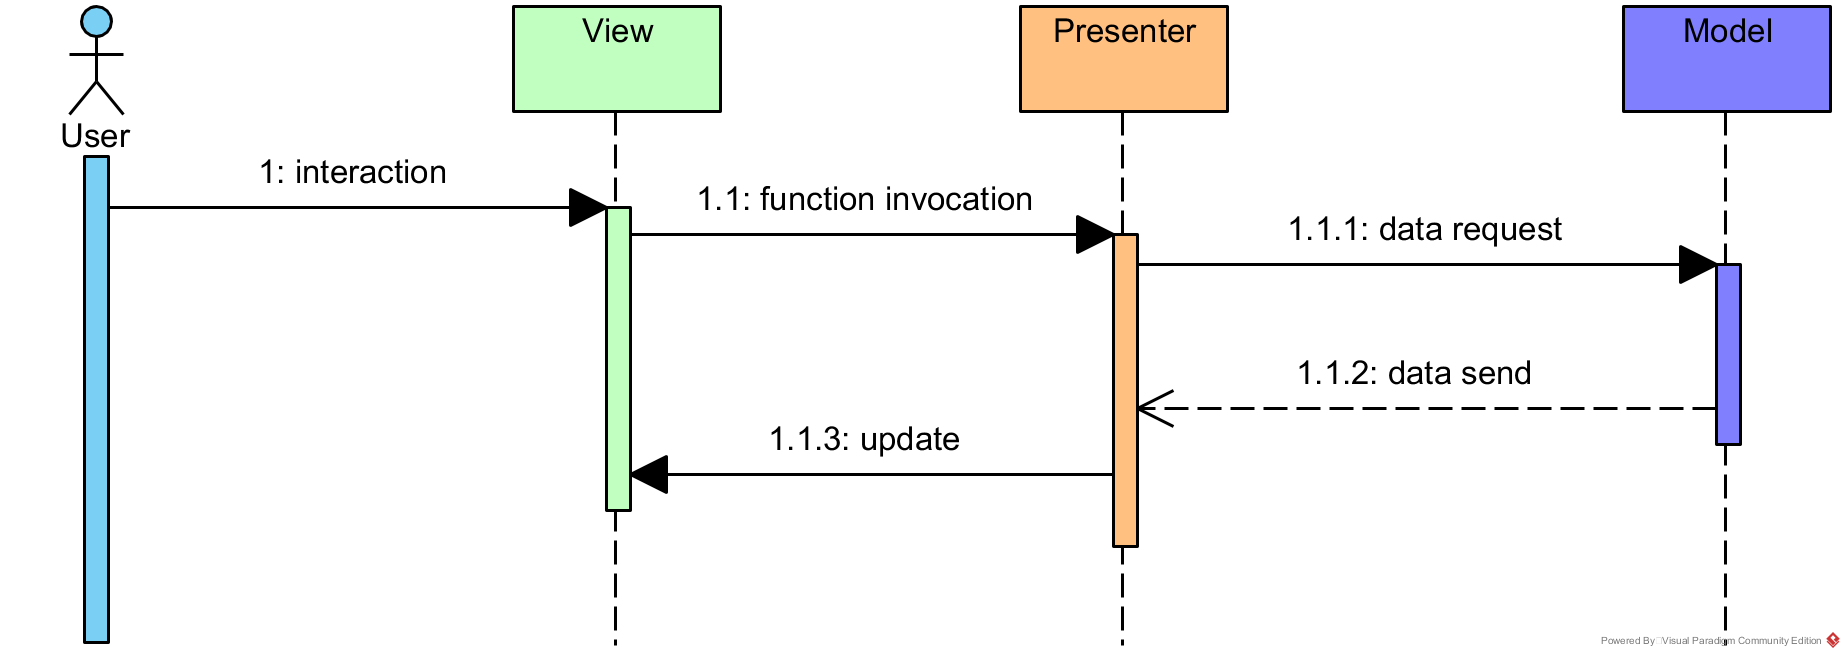
\includegraphics[width=\columnwidth]{progettazione/mvpSequenceDiagram} 
    \caption{Diagramma di sequenza del \textit{pattern} \textit{MVP}}
\end{figure}

Importanti vantaggi nell'utilizzo del \textit{pattern} \textit{MVP} sono:
\begin{itemize}
	\item possibilità di utilizzare lo stesso \textit{model} da parte di \textit{view} differenti;
	\item semplicità nell'aggiunta di nuovi tipi di \textit{client}: è sufficiente scrivere un \textit{presenter} e una \textit{view} per ognuna delle nuove applicazioni. Il \textit{pattern} permette quindi un disaccoppiamento tra logica applicativa e \textit{database} sottostante.
\end{itemize}

\subsection{Architettura \textit{back end}}

Il \textit{server} presenta un'\glossaryItem{architettura a strati} dove i componenti sono organizzati in strati orizzontali, ed ognuno di questi possiede specifici ruoli e responsabilità nel contesto dell'applicazione. Nel contesto del progetto il \textit{pattern} è stato diviso nei seguenti strati:
\begin{itemize}
	\item \textbf{\textit{business layer}}: contiene gli oggetti \textit{servlet} del servizio \textit{web}, i quali si occupano di captare le richieste \textit{HTTP} provenienti dal \textit{client}, di leggere o scrivere sul \textit{database} di conseguenza, e di fornire delle risposte;
	\item \textbf{\textit{persistance layer}}: contiene le classi del servizio \textit{web} che permettono agli oggetti \textit{servlet} di accedere al \textit{database} dell'applicazione;
	\item \textbf{\textit{database layer}}: contiene i \textit{database} dell'applicazione.
\end{itemize}

\newpage

Viene di seguito presentata una figura illustrativa di come il \textit{layered architecture pattern} è stato istanziato nel \glossaryItem{back end} di \textit{moviORDER}. 

\begin{figure}[!h] 
    \centering 
    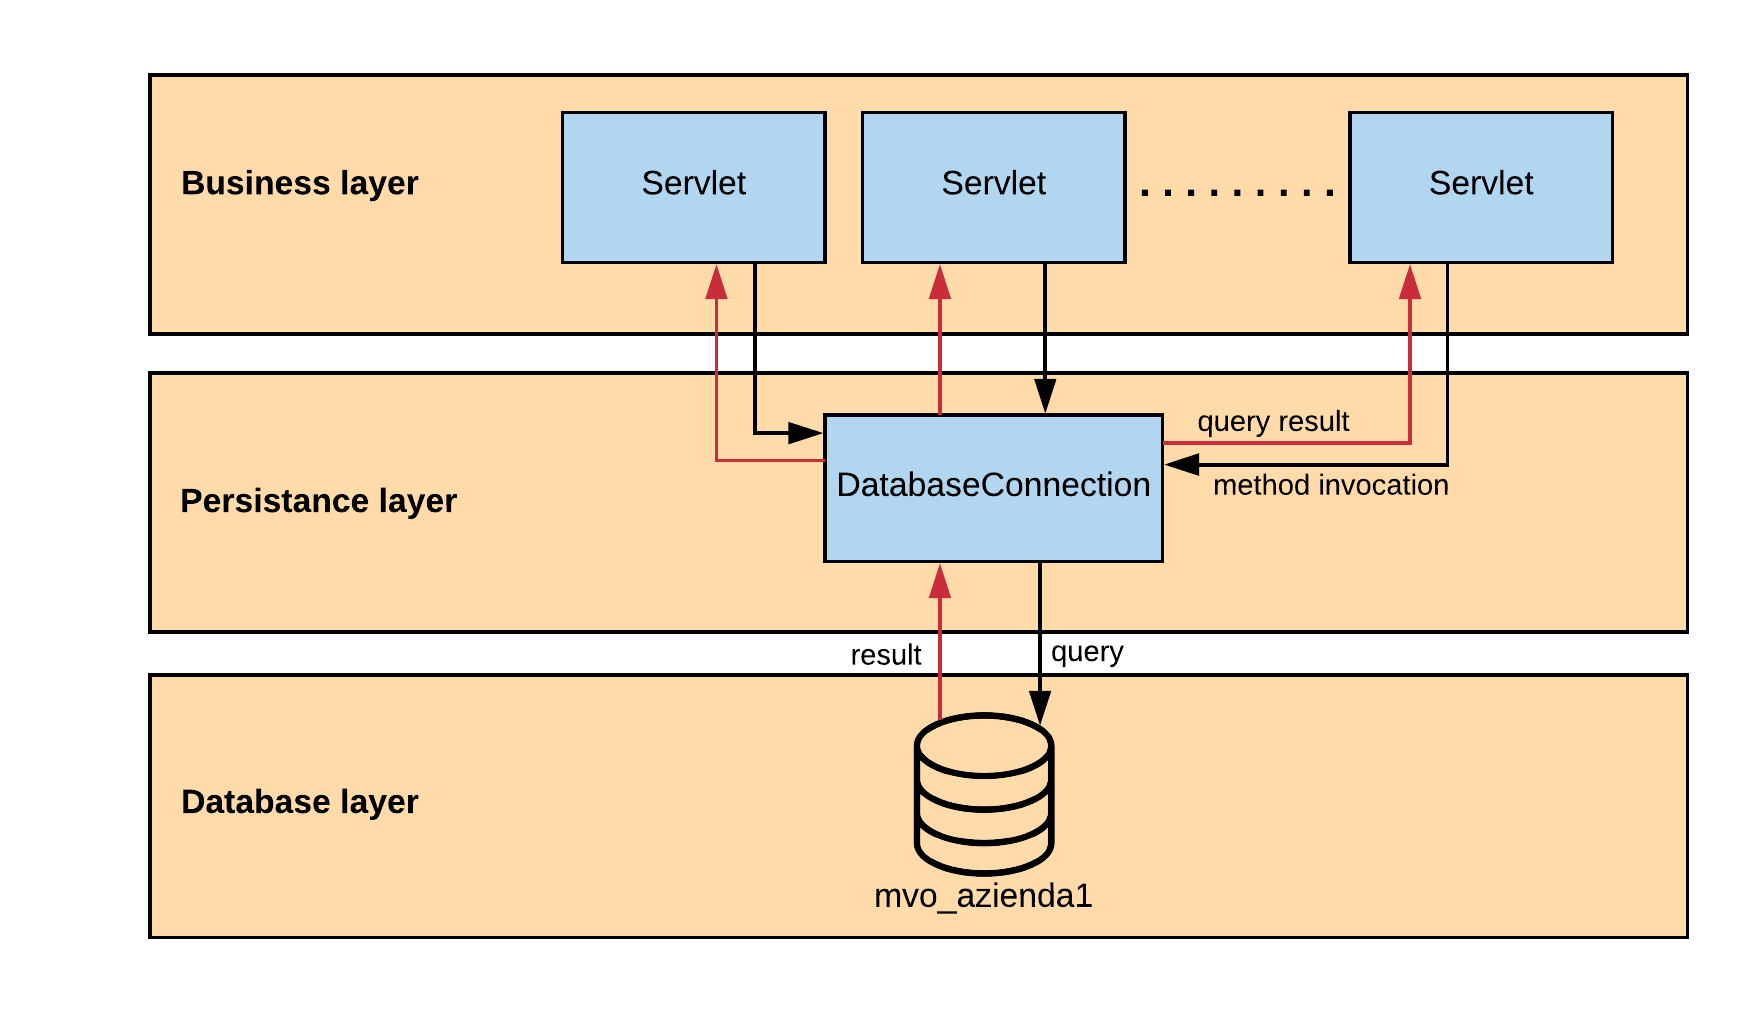
\includegraphics[width=\columnwidth]{progettazione/serverArchitecture} 
    \caption{Architettura a strati del \textit{back end}}
\end{figure}

Uno dei vantaggi dell'architettura a strati è la separazione delle responsabilità tra i componenti. Un componente all'interno di uno specifico strato può eseguire solamente compiti che spettano allo stesso. Questo tipo di classificazione facilita lo sviluppo, il \textit{testing} e la manutenzione del \textit{back end}.

\newpage

\section{Progettazione servizio \textit{web}}

Il seguente diagramma dei \textit{package} rappresenta la struttura del servizio \textit{web} di \textit{moviORDER}.

\begin{figure}[!h] 
    \centering 
    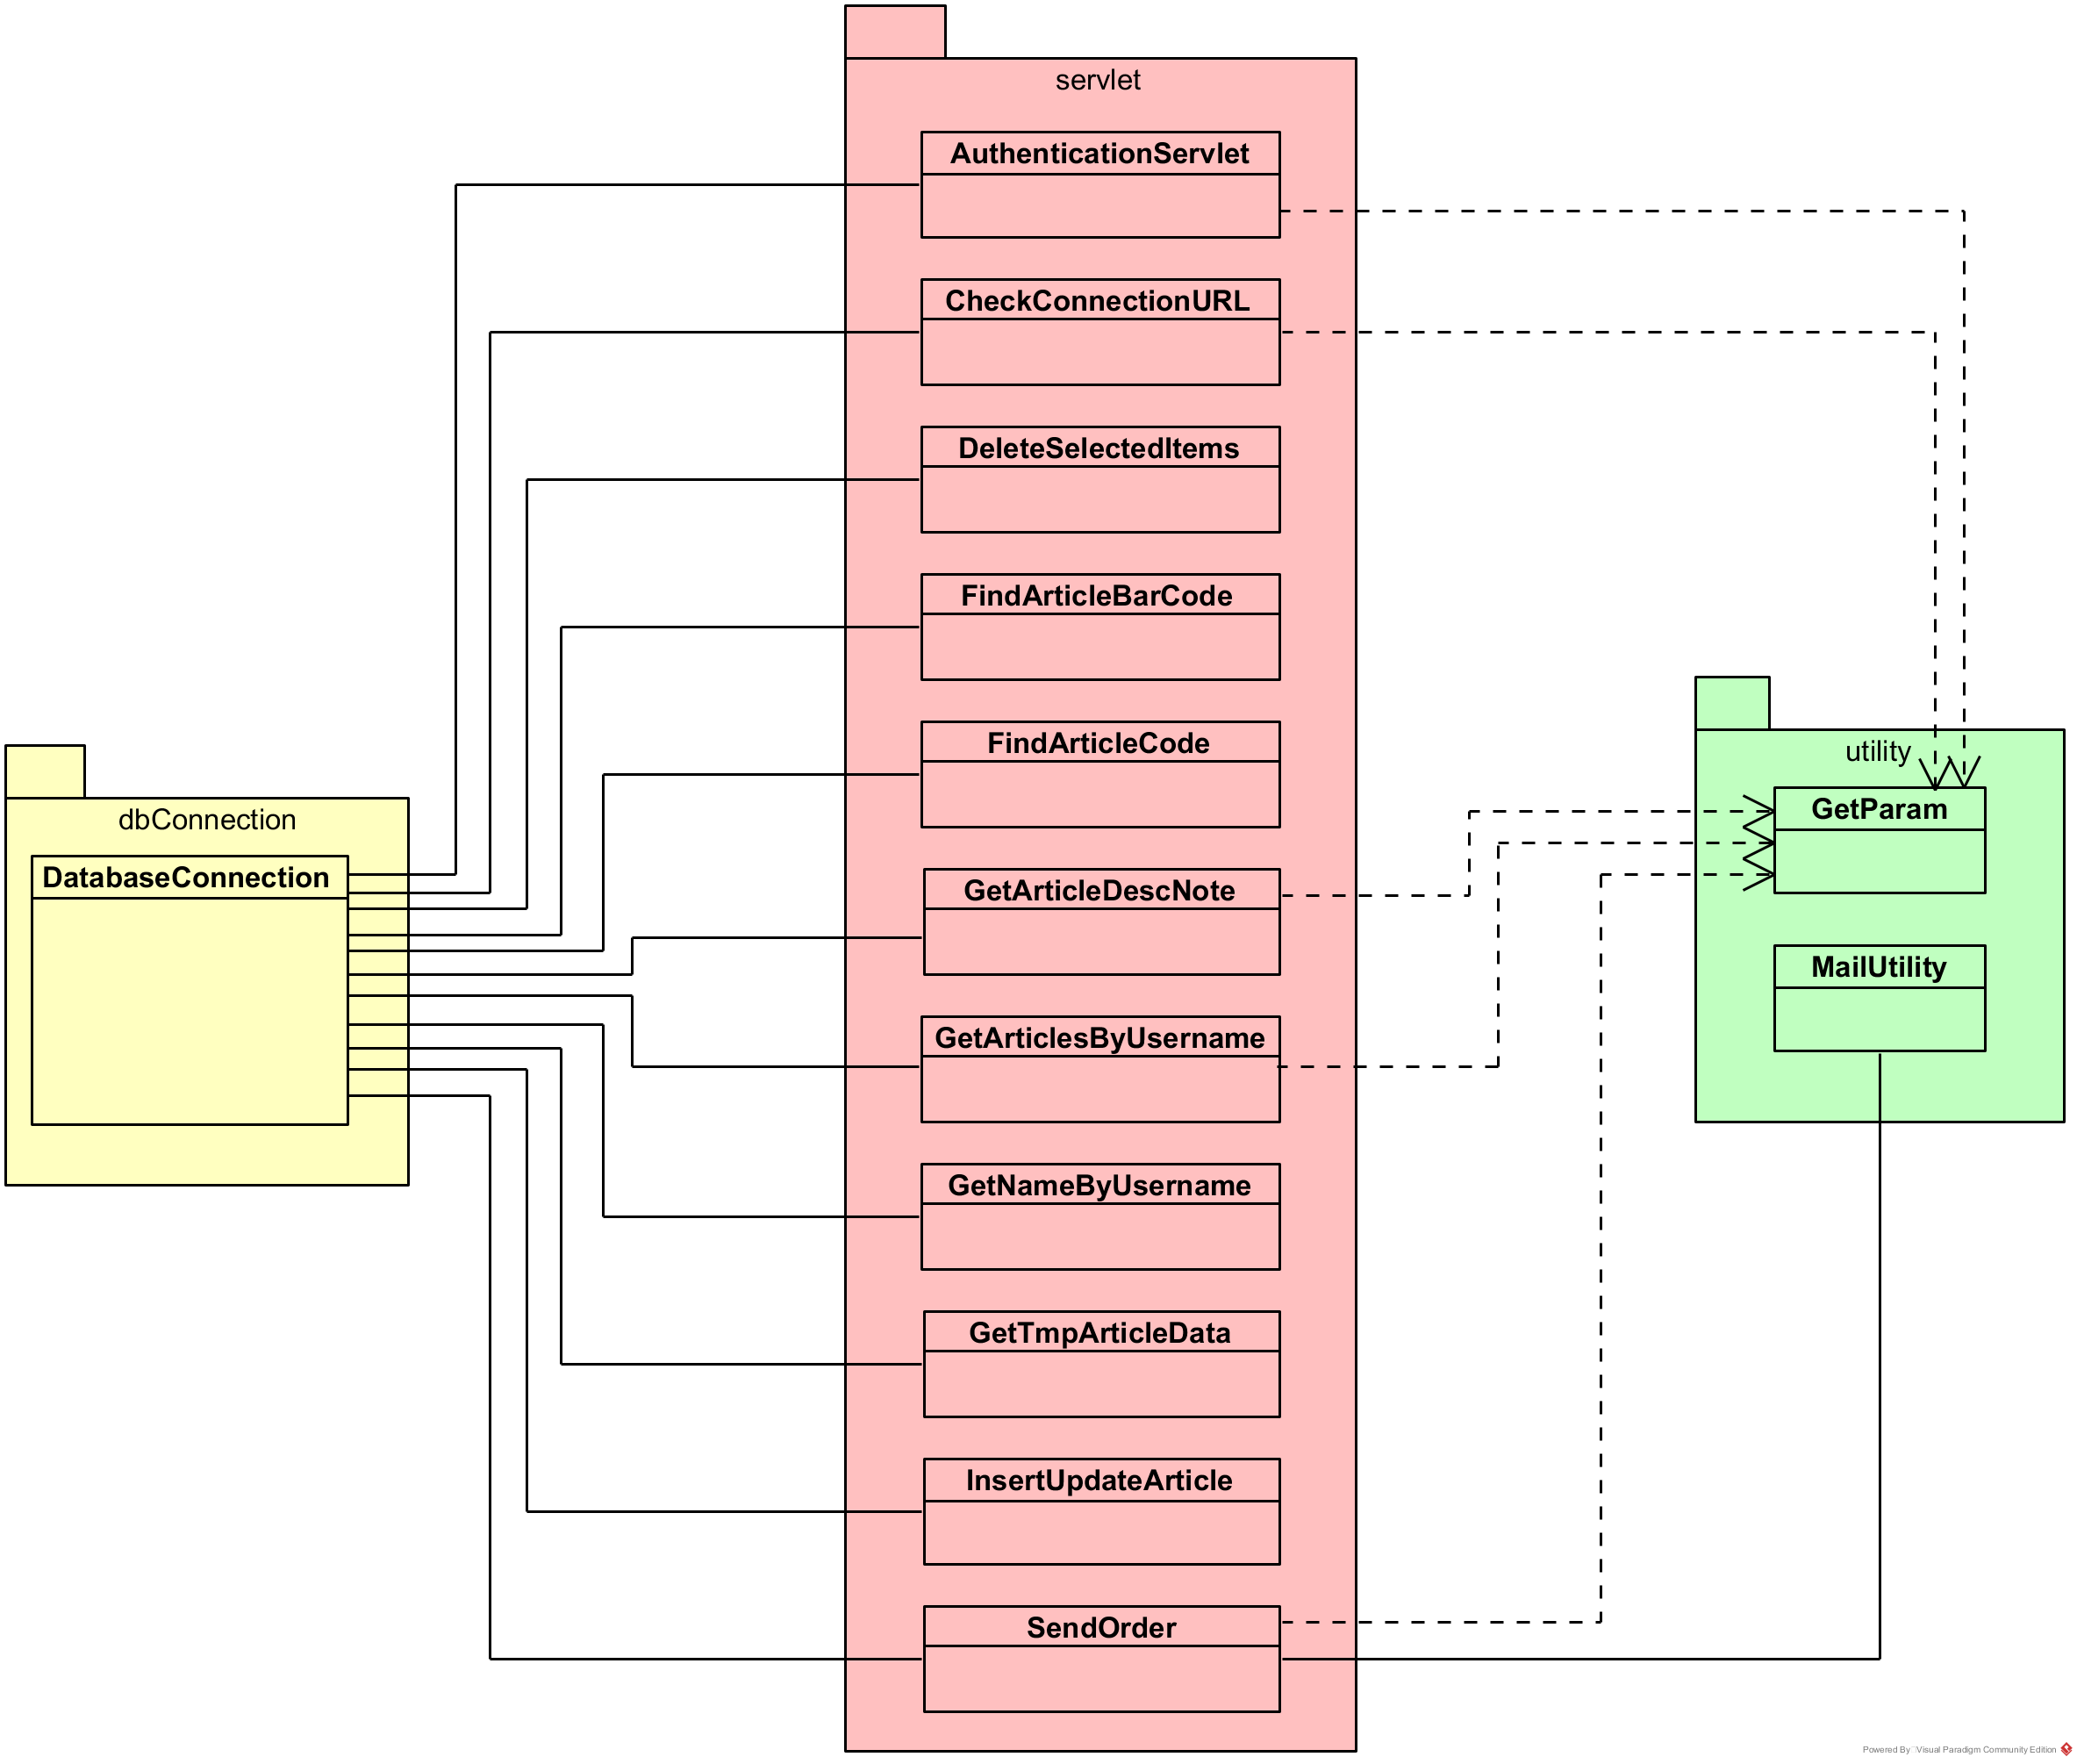
\includegraphics[width=\columnwidth]{progettazione/packages} 
    \caption{Diagramma dei \textit{package} del servizio \textit{web}}
\end{figure}

Come si può vedere dal diagramma, il servizio è costituito da tre \textit{package}:
\begin{itemize}
	\item \textit{dbConnection}: contiene classi atte alla gestione della connessione con un \textit{database}. Il \textit{package} viene utilizzato per permettere agli oggetti \textit{servlet} di connettersi a \textit{database} \textit{SQL Server} locali o remoti;
	\item \textit{servlet}: contiene le classi che definiscono gli oggetti \textit{servlet} del servizio. Essi si occupano di captare le richieste \textit{HTTP} provenienti dal \textit{client} e di rispondere a queste tramite stringhe in formato \textit{JSON};
	\item \textit{utility}: contiene le classi utilità del servizio. Esse facilitano i compiti che gli oggetti \textit{servlet} devono eseguire.
\end{itemize}
Una descrizione più approfondita di come tali \textit{package} sono stati utilizzati nella codifica del servizio \textit{web} è presente in sezione §\ref{codificaservizio}.

\subsection{\textit{Package servlet}}

Essendo il \textit{package} \textit{servlet} il più articolato, merita una descrizione più approfondita. Il seguente diagramma delle classi rappresenta la struttura del \textit{package} \textit{servlet}.

\begin{figure}[!h] 
    \centering 
    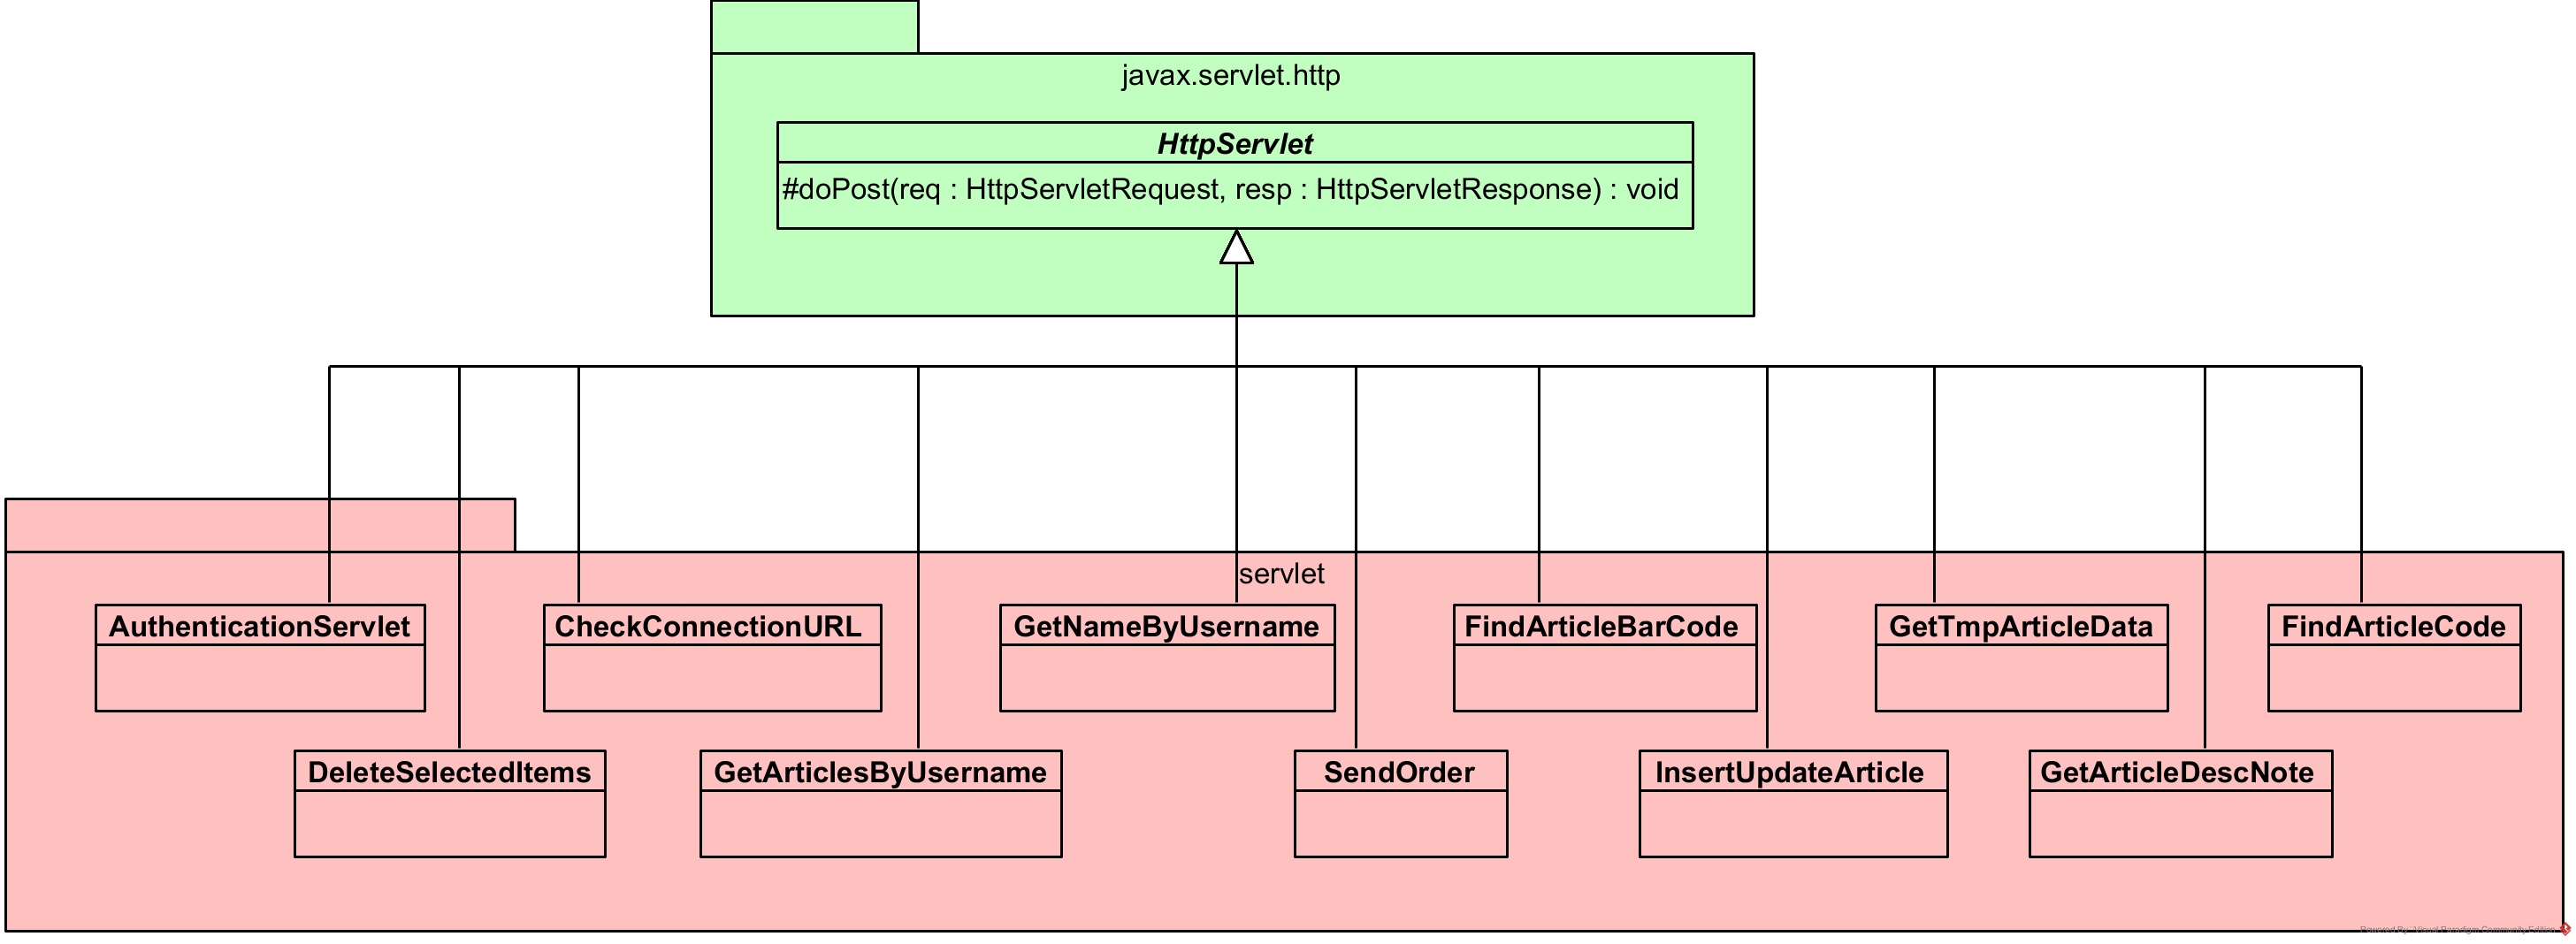
\includegraphics[width=\columnwidth]{progettazione/servletPackage} 
    \caption{Diagramma delle classi del \textit{package} \textit{servlet}}
\end{figure}

Come si può vedere dal diagramma, ogni classe \textit{servlet} concreta eredita dalla classe astratta \textit{HttpServlet}. Inoltre, ogni \textit{servlet} concreto definisce il metodo \textit{doPost()}, il quale permette di definire il comportamento del \textit{servlet} alla ricezione di richieste \textit{HTTP POST}. Una descrizione di come queste classi sono state implementate nella pratica è presente in sezione §\ref{codificaservizio}.

\section{Progettazione \textit{database}} \label{progdb}

Come detto precedentemente, i dati di \textit{moviORDER} sono raggruppati all'interno di due \textit{database}. Il \textit{database} \textit{CommonDb} contiene i dati di autenticazione degli utenti di \textit{moviORDER} e le stringhe di connessione ai rispettivi \textit{database} aziendali (ogni azienda possiede un proprio \textit{database}), mentre il \textit{database} \textit{mvo\_aziendaNomeAzienda} contiene tutti i dati utili alla gestione degli ordini presso l'azienda \textit{NomeAzienda}. In fase di autenticazione, le credenziali dell'utente vengono cercate all'interno del \textit{CommonDb} e, in caso di corrispondenza, viene prelevata la stringa di connessione al \textit{database} dell'azienda presso cui l'utente è cliente. Successivamente, questa viene utilizzata per collegare l'applicazione al \textit{database} corretto, permettendo all'utente di visualizzare solamente i dati sugli articoli venduti dalla propria azienda.
Il \textit{database} \textit{CommonDb} presenta le seguenti tabelle:
\begin{itemize}
	\item \textbf{Users}: tabella contenente i dati di autenticazione degli utenti di \textit{moviORDER}. La tabella presenta i seguenti campi:
		\begin{itemize}
			\item \textit{UserName} (\glossaryItem{chiave primaria}): è il nome utente per accedere all'applicazione. Viene reso univoco poiché costituito dalla concatenazione della partita IVA dell'azienda con un codice auto-incrementante assegnato al cliente quando gli viene consegnata l'applicazione;
			\item \textit{Password}: è la \textit{password} per accedere all'applicazione. La coppia \textit{username}/\textit{password} viene assegnata all'utente quando gli viene consegnata l'applicazione;
			\item \textit{CodAzienda} (\glossaryItem{chiave esterna}): è l'identificativo univoco dell'azienda presso cui l'utente è cliente. Questo campo presenta un vincolo d'integrità referenziale con il campo \textit{CodAzienda} della tabella \textbf{Aziende};
			\item \textit{EmailU}: è l'indirizzo \textit{e-mail} dell'utente;
			\item \textit{Bloccato}: è un \textit{flag} che vale 1 se l'utente è stato bloccato dall'azienda, oppure 0 se il suo \textit{account} è attivo.
		\end{itemize}
	\item \textbf{Aziende}: tabella contenente le stringhe di connessione ai \textit{database} aziendali di tutte le aziende registrate al servizio \textit{moviORDER}. Contiene inoltre i parametri di configurazione del \textit{server SMTP} di ogni azienda, il quale viene utilizzato da \textit{moviORDER} per inviare le \textit{mail} di conferma dei vari ordini registrati. La tabella presenta i seguenti campi:
	\begin{itemize}
		\item \textit{CodAzienda} (chiave primaria): è l'identificativo univoco dell'azienda;
		\item \textit{Path}: è la stringa di connessione al \textit{database} aziendale;
		\item \textit{EmailA}: è l'indirizzo \textit{e-mail} aziendale;
		\item \textit{Host}: è l'indirizzo della macchina dove è installato il \textit{server SMTP} dell'azienda;
		\item \textit{Post}: è la porta su cui è installato il \textit{server SMTP} dell'azienda;
		\item \textit{Username}: è il nome utente per accedere al \textit{server SMTP} dell'azienda;
		\item \textit{Password}: è la \textit{password} per accedere al \textit{server SMTP} dell'azienda.
	\end{itemize}
\end{itemize}
Viene di seguito presentato il diagramma \textit{ER} del \textit{database} \textit{CommonDb}. Le chiavi primarie sono sottolineate, mentre quelle esterne sono scritte in corsivo.

\begin{figure}[!h] 
    \centering 
    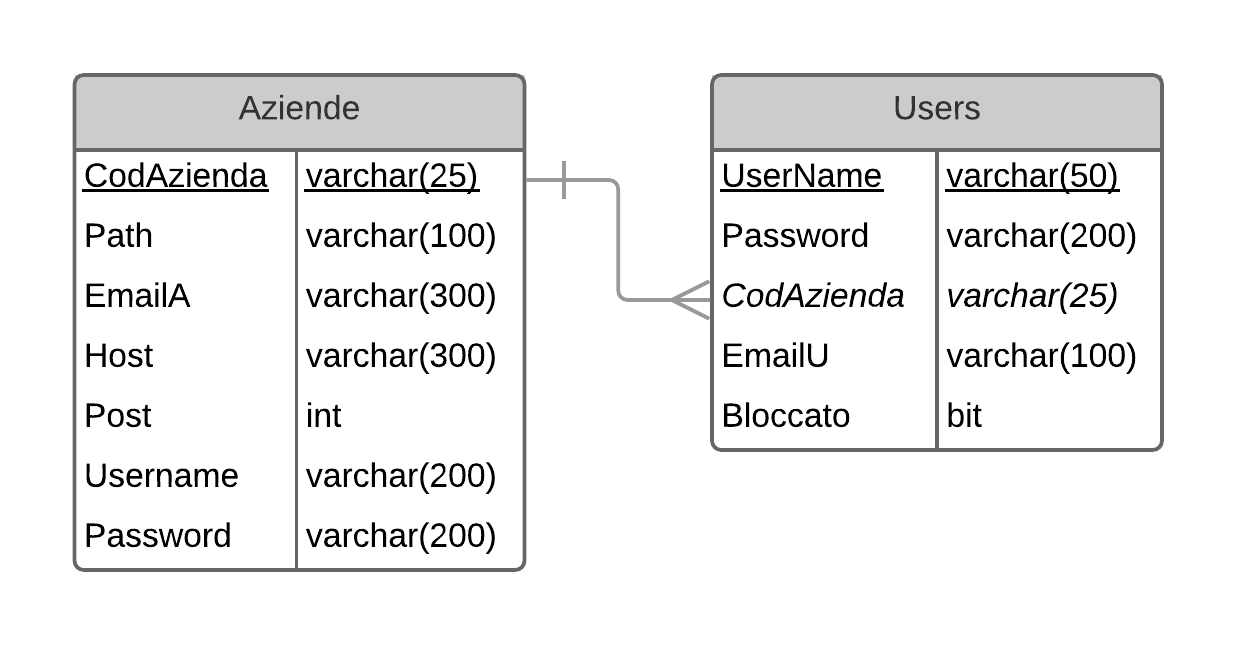
\includegraphics[width=\columnwidth]{progettazione/erCommon} 
    \caption{Diagramma \textit{ER} del \textit{database} \textit{CommonDb}}
\end{figure}

\newpage

Il \textit{database} \textit{mvo\_aziendaNomeAzienda} presenta le seguenti tabelle:
\begin{itemize}
	\item \textbf{Art}: tabella contenente i dati sugli articoli venduti dall'azienda \textit{NomeAzienda}. La tabella presenta i seguenti campi:
		\begin{itemize}
			\item \textit{Id\_Art}: è un codice auto-incrementante assegnato al \textit{record};
			\item \textit{CodArt} (chiave primaria): è il codice dell'articolo, che lo identifica univocamente;
			\item \textit{DesArt}: è il nome dell'articolo;
			\item \textit{Note}: sono le note presenti in \textit{database} per l'articolo;
			\item \textit{QtaMin}: è la minima quantità ordinabile per l'articolo;
			\item \textit{QtaMul}: è lo \textit{step} di quantità ordinabile per l'articolo. Ad esempio se \textit{QtaMul} è 2, significa che è possibile ordinare 2, 4, 6 pezzi dell'articolo, e così via.
		\end{itemize}
	\item \textbf{ArtAlias}: tabella contenente i codici a barre degli articoli venduti dall'azienda. La tabella presenta i seguenti campi:
		\begin{itemize}
			\item \textit{Id\_ArtAlias}: è un codice auto-incrementante assegnato al \textit{record};
			\item \textit{CodArt} (chiave primaria, chiave esterna): è il codice dell'articolo. Questo campo presenta un vincolo d'integrità referenziale con il campo \textit{CodArt} della tabella \textbf{Art};
			\item \textit{Alias} (chiave primaria): è il codice a barre dell'articolo. Questo campo fa parte della chiave primaria, insieme a \textit{CodArt}, poiché è possibile che un articolo abbia più codici a barre.
		\end{itemize}
	\item \textbf{DocRig}: tabella contenente i dati d'ordine degli articoli che sono stati ordinati presso l'azienda. La tabella presenta i seguenti campi:
		\begin{itemize}
			\item \textit{Id\_DocRig} (chiave primaria): è un codice auto-incrementante assegnato al \textit{record}; 
			\item \textit{Id\_DocTes} (chiave esterna): è il codice della fattura a cui il prodotto ordinato appartiene. Questo campo presenta un vincolo di integrità referenziale con il campo \textit{Id\_DocTes} della tabella \textbf{DocTes};
			\item \textit{Username} (chiave esterna): è il nome utente dell'utente che ha ordinato l'articolo. Questo campo presenta un vincolo d'integrità referenziale con il campo \textit{UserID} della tabella \textbf{Users};
			\item \textit{CodArt} (chiave esterna): è il codice dell'articolo ordinato. Questo campo presenta un vincolo d'integrità referenziale con il campo \textit{CodArt} della tabella \textbf{Art};
			\item \textit{Quantita}: è la quantità ordinata dell'articolo;
			\item \textit{Note}: sono le note che l'utente ha inserito per l'articolo quando l'ha aggiunto al carrello.
		\end{itemize}
	\item \textbf{DocTes}: tabella contenente i dati delle fatture degli ordini che sono stati registrati prezzo l'azienda. La tabella presenta i seguenti campi:
		\begin{itemize}
			\item \textit{Id\_DocTes} (chiave primaria): è un codice auto-incrementante assegnato al \textit{record};
			\item \textit{CodDoc} (chiave esterna): è un codice che rappresenta la tipologia di fattura emessa dall'azienda. Questo campo presenta un vincolo d'integrità referenziale con il campo \textit{CodDoc} della tabella \textbf{Users};
			\item \textit{CodCliFor}: è il nome utente dell'utente che ha eseguito l'ordine presso l'azienda;
			\item \textit{DataDoc}: è la data dell'ordine;
			\item \textit{Note}: sono le note inserite dall'utente in fase di invio ordine;
			\item \textit{Status}: è un \textit{flag} che vale 0 nel momento in cui il \textit{record} viene memorizzato in tabella, 1 quando inizia l'importazione dello stesso verso il gestionale di \visione{}, e 2 quando l'importazione è terminata.
		\end{itemize}
	\item \textbf{TmpRig}: tabella contenente i dati d'ordine degli articoli presenti nel carrello degli utenti dell'azienda. Questi dati servono all'applicazione per tenere memoria del carrello degli utenti. La tabella presenta i seguenti campi:
		\begin{itemize}
			\item \textit{Id\_TmpRig} (chiave primaria): è un codice auto-incrementante assegnato al \textit{record};
			\item \textit{Username} (chiave esterna): è il nome utente dell'utente che presenta l'articolo in carrello. Questo campo presenta un vincolo d'integrità referenziale con il campo \textit{UserID} della tabella \textbf{Users};
			\item \textit{CodArt} (chiave esterna): è il codice dell'articolo. Questo campo presenta un vincolo d'integrità referenziale con il campo \textit{CodArt} della tabella \textbf{Art};
			\item \textit{Quantita}: è la quantità che l'utente ha inserito per l'articolo quando l'ha aggiunto al carrello;
			\item \textit{Note}: sono le note che l'utente ha inserito per l'articolo quando l'ha aggiunto al carrello.
		\end{itemize}
	\item \textbf{Users}: tabella contenente le informazioni anagrafiche degli utenti dell'azienda. Essa presenta i seguenti campi:
		\begin{itemize}
			\item \textit{UserID} (chiave primaria): è il nome utente dell'utente;
			\item \textit{DesCliFor}: è una breve descrizione dell'utente;
			\item \textit{Indirizzo}: è l'indirizzo di residenza dell'utente;
			\item \textit{Localita}: è la località di residenza dell'utente;
			\item \textit{CodProv}: è il codice della provincia di residenza dell'utente;
			\item \textit{CodNazione}: è il codice della nazione di residenza dell'utente;
			\item \textit{CodDoc}: è il codice della fattura che deve essere emessa quando l'utente effettua un ordine;
			\item \textit{DesDoc}: è una descrizione della fattura che deve essere emessa quando l'utente effettua un ordine.
		\end{itemize}
\end{itemize}
Viene di seguito presentato il diagramma \textit{ER} del \textit{database} \textit{mvo\_aziendaNomeAzienda}. Le chiavi primarie sono sottolineate, mentre quelle esterne sono scritte in corsivo.

\begin{figure}[!h] 
    \centering 
    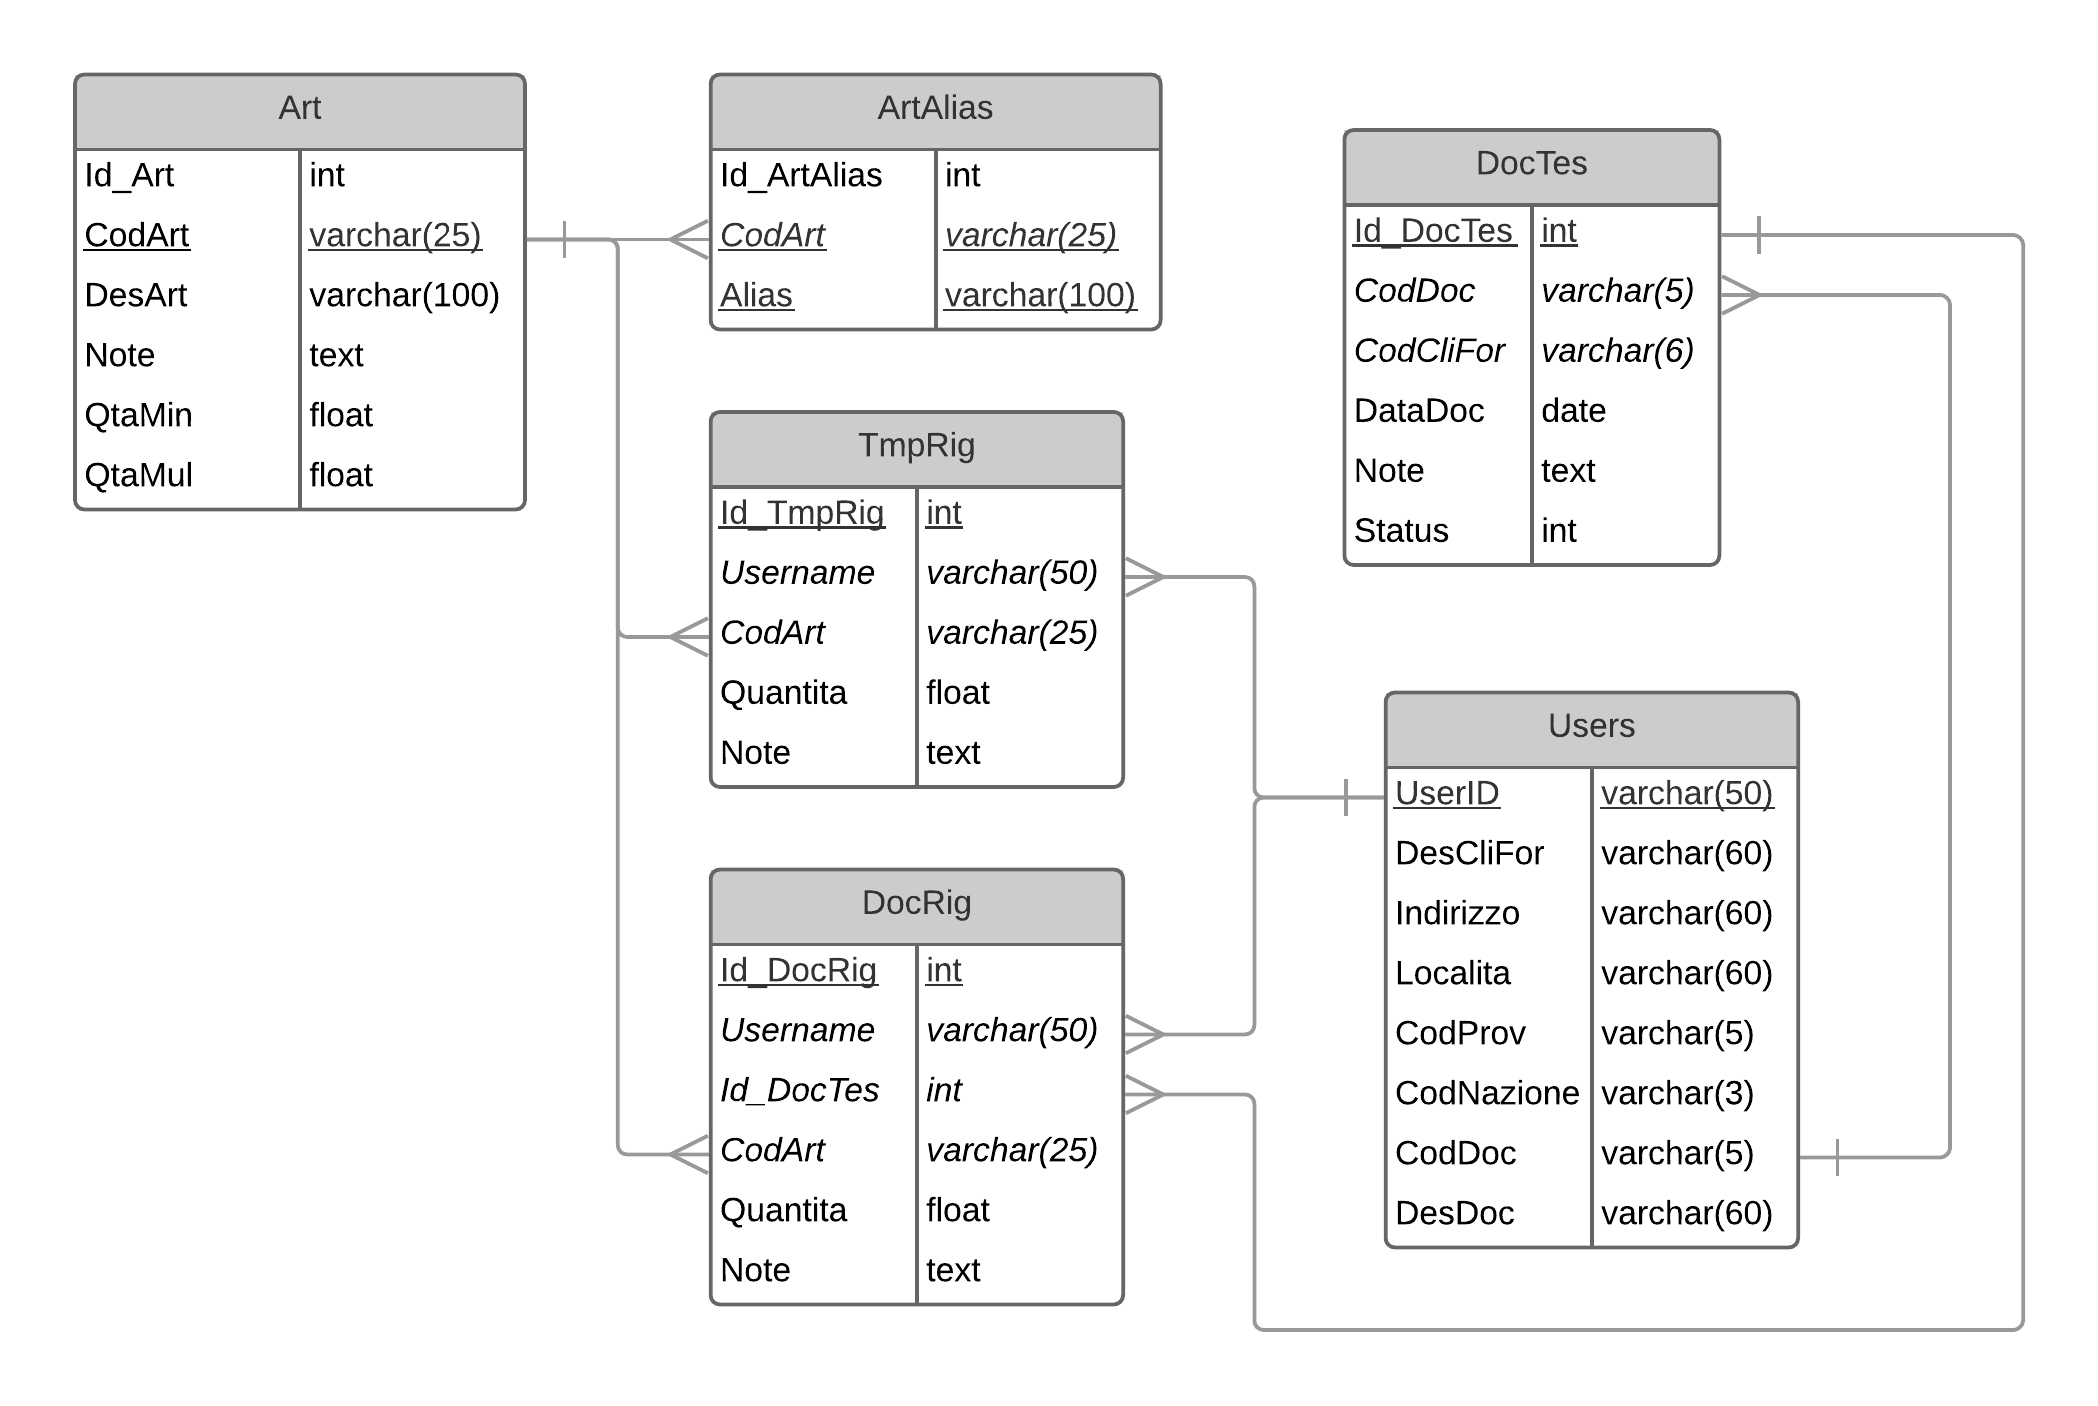
\includegraphics[width=\columnwidth]{progettazione/erMvoAzienda} 
    \caption{Diagramma \textit{ER} del \textit{database} \textit{mvo\_aziendaNomeAzienda}}
\end{figure}

